<<<<<<< Updated upstream
\documentclass[12pt]{report} % Times New Roman, 12pt
%\usepackage{gscale_thesis_singlespace} % Single spaced thesis
\usepackage{gscale_thesis_doublespace} % Double spaced thesis
\usepackage{fancyheadings} % Header and footer styling
\usepackage{natbib} % Bibliography formatting
\usepackage{setspace} % Allows double spacing but skips headers/footers
\setcounter{tocdepth}{1} % Limits the TOC to chapter and section names

% Additional packages
\usepackage{graphicx} % Allows the inclusion of figures
\usepackage{subcaption} % Allows captions to be added to subfigures
\usepackage[justification=centering]{caption} % Centres caption text
\usepackage{array} % Used for table formatting
\newcolumntype{P}[1]{>{\raggedright\let\newline\\\arraybackslash\hspace{0pt}}m{#1}}
\usepackage{booktabs} % Fancy-style tables
\usepackage{longtable} % Allows for tables that are more than one page long
\usepackage{float} % Better figure placement control
\usepackage{enumerate} % Numbered lists
\usepackage[shortlabels]{enumitem} % For controlling enumerate labels
\usepackage[shortcuts]{extdash} % Allows manual hyphenation of hypenated words
\usepackage{amsmath} % Non-standard math symbols
\usepackage{amsfonts} % Extended fonts for mathematics

\usepackage[hidelinks]{hyperref} % Linking to LaTeX labels and external URLs

\numberwithin{equation}{section} % Numbers equations based on their section

% ********************************
\begin{document}
<<<<<<< Updated upstream
\title{Your Thesis Title, Which Can Be As Long As You Want On the Title Page}
\halftitle{Short Title} % 60 Characters Max. Including Spaces

\author{Jane Doe}
\shortauthor{J. Doe} % Used for page header

\dept{Department You Belong To}
\field{Your Field} % What field your thesis is in (e.g. Software Engineering)

\prevdegreeone{B.Eng. (Software Engineering \& Game Design),\\ McMaster University, Hamilton, Canada}
\prevdegreetwo{B.Eng.} % Just your degree's field

\submitdate{MONTH YEAR} % Use the month's full spelling e.g. November
\copyrightyear{YYYY} % Year you are submitting this, usually your graduation 
%year

\doctype{Report} % ``Report'' or ``Thesis'' or whatever you need
\degree{Masters of Engineering} % The degree you get when you submit this
\degreeabbrv{M.Eng.}
\principaladviser{Your Supervisor} % Your Supervisor
=======
<<<<<<< HEAD
\title{Your Thesis Title, Which Can Be As Long As You Want On the Title Page}
\halftitle{Short Title} % 60 Characters Max. Including Spaces

\author{Jane Doe}
\shortauthor{J. Doe} % Used for page header

\dept{Department You Belong To}
\field{Your Field} % What field your thesis is in (e.g. Software Engineering)

\prevdegreeone{B.Eng. (Software Engineering \& Game Design),\\ McMaster University, Hamilton, Canada}
\prevdegreetwo{B.Eng.} % Just your degree's field

\submitdate{MONTH YEAR} % Use the month's full spelling e.g. November
\copyrightyear{YYYY} % Year you are submitting this, usually your graduation 
%year

\doctype{Report} % ``Report'' or ``Thesis'' or whatever you need
\degree{Masters of Engineering} % The degree you get when you submit this
\degreeabbrv{M.Eng.}
\principaladviser{Your Supervisor} % Your Supervisor
=======
\title{Your Thesis Title, Which Can Be As Long As You Want On the Title Page}
\halftitle{Short Title} % 60 Characters Max. Including Spaces

\author{Jane Doe}
\shortauthor{J. Doe} % Used for page header

\dept{Department You Belong To}
\field{Your Field} % What field your thesis is in (e.g. Software Engineering)

\prevdegreeone{B.Eng. (Software Engineering \& Game Design),\\ McMaster University, Hamilton, Canada}
\prevdegreetwo{B.Eng.} % Just your degree's field

\submitdate{MONTH YEAR} % Use the month's full spelling e.g. November
\copyrightyear{YYYY} % Year you are submitting this, usually your graduation 
%year

\doctype{Report} % ``Report'' or ``Thesis'' or whatever you need
\degree{Masters of Engineering} % The degree you get when you submit this
\degreeabbrv{M.Eng.}
\principaladviser{Your Supervisor} % Your Supervisor
>>>>>>> 9d845fd9678a4217417e588c8e1f2a2f78b24c2f
>>>>>>> Stashed changes
 % LaTeX variables for preface pages/headers
    
\beforepreface % Half title page, title page, declaration page   
  <<<<<<< Updated upstream
\prefacesection{Lay Abstract}

=======
<<<<<<< HEAD
\prefacesection{Lay Abstract}

=======
\prefacesection{Lay Abstract}

>>>>>>> 9d845fd9678a4217417e588c8e1f2a2f78b24c2f
>>>>>>> Stashed changes
A lay abstract of not more 150 words must be included explaining the key goals and contributions of the thesis in lay terms that is accessible to the general public.  % Lay Abstract
  <<<<<<< Updated upstream
\prefacesection{Abstract}

=======
<<<<<<< HEAD
\prefacesection{Abstract}

=======
\prefacesection{Abstract}

>>>>>>> 9d845fd9678a4217417e588c8e1f2a2f78b24c2f
>>>>>>> Stashed changes
Abstract here (no more than 300 words) % Abstract
  <<<<<<< Updated upstream
%\thispagestyle{empty}
\null\vfill
\begin{center}
%\textbf{Dedications}
%\linebreak
\textsl{Your Dedication \\ Optional second line}
\end{center}
\vfill
=======
<<<<<<< HEAD
%\thispagestyle{empty}
\null\vfill
\begin{center}
%\textbf{Dedications}
%\linebreak
\textsl{Your Dedication \\ Optional second line}
\end{center}
\vfill
=======
%\thispagestyle{empty}
\null\vfill
\begin{center}
%\textbf{Dedications}
%\linebreak
\textsl{Your Dedication \\ Optional second line}
\end{center}
\vfill
>>>>>>> 9d845fd9678a4217417e588c8e1f2a2f78b24c2f
>>>>>>> Stashed changes
 % Dedication
  <<<<<<< Updated upstream
\prefacesection{Acknowledgements}

=======
<<<<<<< HEAD
\prefacesection{Acknowledgements}

=======
\prefacesection{Acknowledgements}

>>>>>>> 9d845fd9678a4217417e588c8e1f2a2f78b24c2f
>>>>>>> Stashed changes
Acknowledgements go here. % Acknowledgements
  \referencepages % Table of Contents, List of Figures, List of Tables
  <<<<<<< Updated upstream
\prefacesection{Notation, Definitions, and Abbreviations}

\section*{Notation}
\begin{description}[font=\rmfamily\bfseries, leftmargin=3cm, style=nextline]
	\item[$A \leq B$] A is less than or equal to B
\end{description}

\section*{Definitions}
\begin{description}[font=\rmfamily\bfseries, leftmargin=3cm, style=nextline]
	\item[Challenge] With respect to video games, a challenge is a set of goals presented to the player that they are tasks with completing; challenges can test a variety of player skills, including accuracy, logical reasoning, and creative problem solving
\end{description}

\section*{Abbreviations}
\begin{description}[font=\rmfamily\bfseries, leftmargin=3cm, style=nextline]
	\item[AI] Artificial intelligence
=======
<<<<<<< HEAD
\prefacesection{Notation, Definitions, and Abbreviations}

\section*{Notation}
\begin{description}[font=\rmfamily\bfseries, leftmargin=3cm, style=nextline]
	\item[$A \leq B$] A is less than or equal to B
\end{description}

\section*{Definitions}
\begin{description}[font=\rmfamily\bfseries, leftmargin=3cm, style=nextline]
	\item[Challenge] With respect to video games, a challenge is a set of goals presented to the player that they are tasks with completing; challenges can test a variety of player skills, including accuracy, logical reasoning, and creative problem solving
\end{description}

\section*{Abbreviations}
\begin{description}[font=\rmfamily\bfseries, leftmargin=3cm, style=nextline]
	\item[AI] Artificial intelligence
=======
\prefacesection{Notation, Definitions, and Abbreviations}

\section*{Notation}
\begin{description}[font=\rmfamily\bfseries, leftmargin=3cm, style=nextline]
	\item[$A \leq B$] A is less than or equal to B
\end{description}

\section*{Definitions}
\begin{description}[font=\rmfamily\bfseries, leftmargin=3cm, style=nextline]
	\item[Challenge] With respect to video games, a challenge is a set of goals presented to the player that they are tasks with completing; challenges can test a variety of player skills, including accuracy, logical reasoning, and creative problem solving
\end{description}

\section*{Abbreviations}
\begin{description}[font=\rmfamily\bfseries, leftmargin=3cm, style=nextline]
	\item[AI] Artificial intelligence
>>>>>>> 9d845fd9678a4217417e588c8e1f2a2f78b24c2f
>>>>>>> Stashed changes
\end{description}
  \academicstatement{academicachievementdeclaration}
\afterpreface
  
  
  <<<<<<< Updated upstream
\chapter{Introduction}

Every thesis needs an introductory chapter

While you're here, you need to go into \texttt{definitions.tex} to set all the 
information needed for the front matter (e.g. title, author) and page 
header/footer.

You will also find the School of Graduate Studies' preparation guide (August 
2021) for theses and reports. I would give it a quick read so you know what's 
=======
<<<<<<< HEAD
\chapter{Introduction}

Every thesis needs an introductory chapter

While you're here, you need to go into \texttt{definitions.tex} to set all the 
information needed for the front matter (e.g. title, author) and page 
header/footer.

You will also find the School of Graduate Studies' preparation guide (August 
2021) for theses and reports. I would give it a quick read so you know what's 
=======
\chapter{Introduction}

Every thesis needs an introductory chapter

While you're here, you need to go into \texttt{definitions.tex} to set all the 
information needed for the front matter (e.g. title, author) and page 
header/footer.

You will also find the School of Graduate Studies' preparation guide (August 
2021) for theses and reports. I would give it a quick read so you know what's 
>>>>>>> 9d845fd9678a4217417e588c8e1f2a2f78b24c2f
>>>>>>> Stashed changes
expected.                  
        \setcounter{figure}{0}
        \setcounter{equation}{0}
        \setcounter{table}{0}
        
  <<<<<<< Updated upstream
\chapter{Your Chapter Title}

This is a sample chapter

If you need to use quotes, type it ``like this''.

\section{Referencing}
These are some sample references to GAMYGDALA~\citep{popescu2014gamygdala} from 
the \texttt{references.bib} file and state effects of 
cognition~\citep{hudlicka2002time} from the \texttt{references\_another.bib} 
file. These references are not in the same .bib file.

\section{Figures}
This is a single image figure (Figure~\ref{fig_singleenv}):

\begin{figure}[ht]
    \centering
    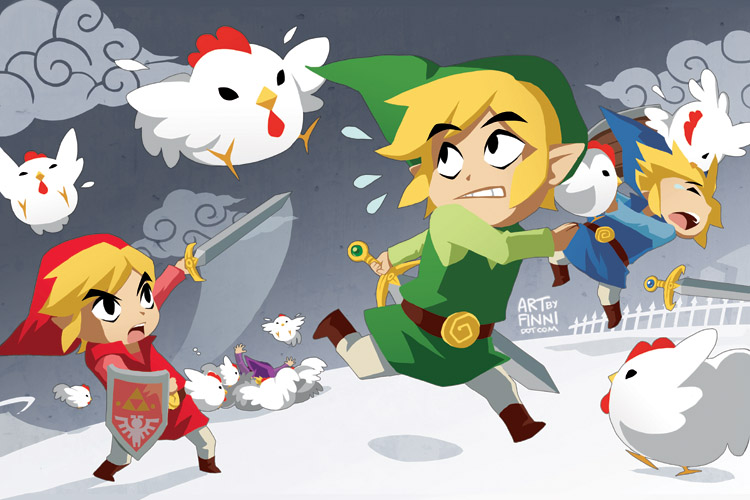
\includegraphics[width=0.6\textwidth]{figures/Sample/tumblr_static_eaceks0rfxsss8o4swscw40wo.jpg}
    \caption[Single Figure Environment Listed Title]{This is a single figure 
    environment}
    \label{fig_singleenv}
\end{figure}

This is a multi-image figure with a top (Figure~\ref{fig_multienv_1}) and bottom (Figure~\ref{fig_multienv_2}) aligned subfigures:

\begin{figure}[ht]
	\centering
	\begin{subfigure}[t]{\textwidth}
		\centering
		
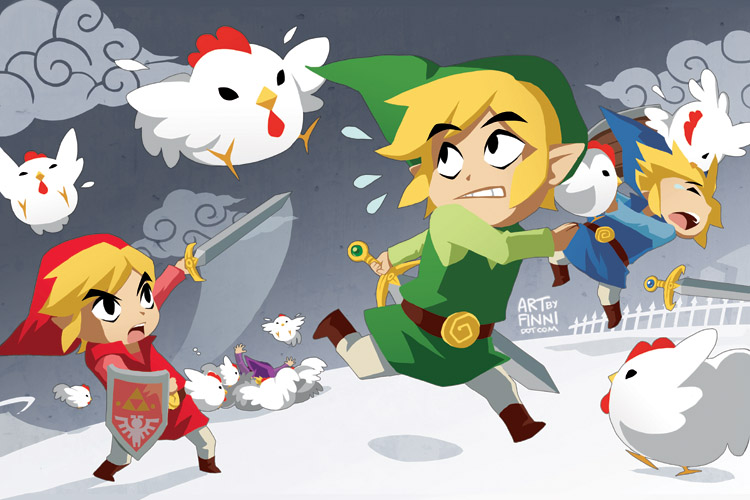
\includegraphics[width=0.7\textwidth]{figures/Sample/tumblr_static_eaceks0rfxsss8o4swscw40wo.jpg}
		\caption{Figure 1}
		\label{fig_multienv_1}
	\end{subfigure}
	~
	\begin{subfigure}[t]{\textwidth}
		\centering
		
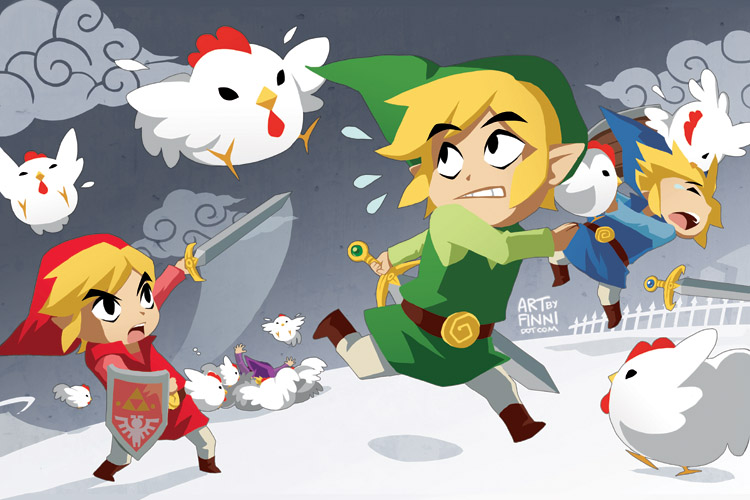
\includegraphics[width=0.7\textwidth]{figures/Sample/tumblr_static_eaceks0rfxsss8o4swscw40wo.jpg}
		\caption{Figure 2}
		\label{fig_multienv_2}
	\end{subfigure}
	
	\caption{A Multi-Figure Environment}
	\label{fig_multienv}
\end{figure}

\section{Tables}

Here is a sample table (Table~\ref{tab_sample}):

	\begin{table}[ht]
	\centering
	\begin{tabular}{ m{0.2\textwidth} m {0.1\textwidth} m{0.15\textwidth} }
		\toprule
		A & $\longleftrightarrow$ & B \\
		C & $\longleftrightarrow$ & D \\
		\bottomrule	
	\end{tabular}	
	\caption{A sample table}	
	\label{tab_sample}
\end{table}

\subsection{Long Tables}
A sample long table is shown in Appendix~\ref{appendix_b}.

\section{Equations}

Here is a sample equation (Equation~\ref{eq_lineslope}):

\begin{equation} \label{eq_lineslope}
	y = mx + b
=======
<<<<<<< HEAD
\chapter{Your Chapter Title}

This is a sample chapter

If you need to use quotes, type it ``like this''.

\section{Referencing}
These are some sample references to GAMYGDALA~\citep{popescu2014gamygdala} from 
the \texttt{references.bib} file and state effects of 
cognition~\citep{hudlicka2002time} from the \texttt{references\_another.bib} 
file. These references are not in the same .bib file.

\section{Figures}
This is a single image figure (Figure~\ref{fig_singleenv}):

\begin{figure}[ht]
    \centering
    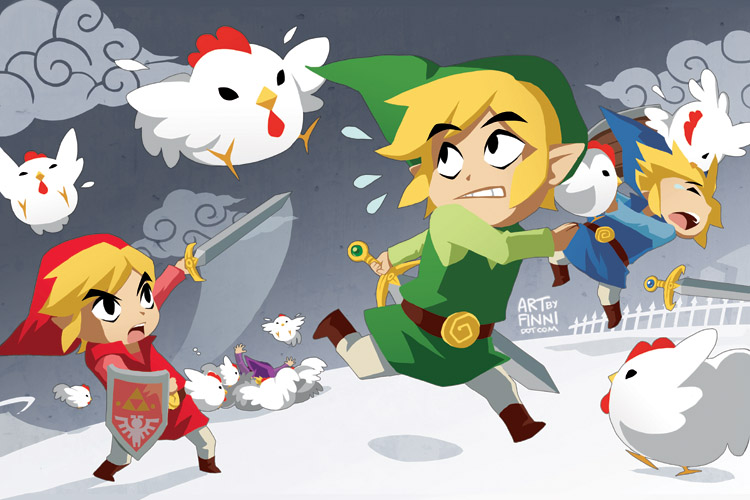
\includegraphics[width=0.6\textwidth]{figures/Sample/tumblr_static_eaceks0rfxsss8o4swscw40wo.jpg}
    \caption[Single Figure Environment Listed Title]{This is a single figure 
    environment}
    \label{fig_singleenv}
\end{figure}

This is a multi-image figure with a top (Figure~\ref{fig_multienv_1}) and bottom (Figure~\ref{fig_multienv_2}) aligned subfigures:

\begin{figure}[ht]
	\centering
	\begin{subfigure}[t]{\textwidth}
		\centering
		
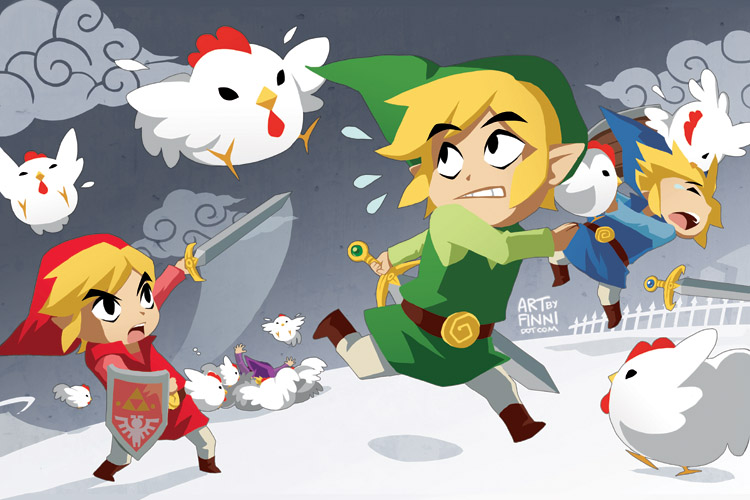
\includegraphics[width=0.7\textwidth]{figures/Sample/tumblr_static_eaceks0rfxsss8o4swscw40wo.jpg}
		\caption{Figure 1}
		\label{fig_multienv_1}
	\end{subfigure}
	~
	\begin{subfigure}[t]{\textwidth}
		\centering
		
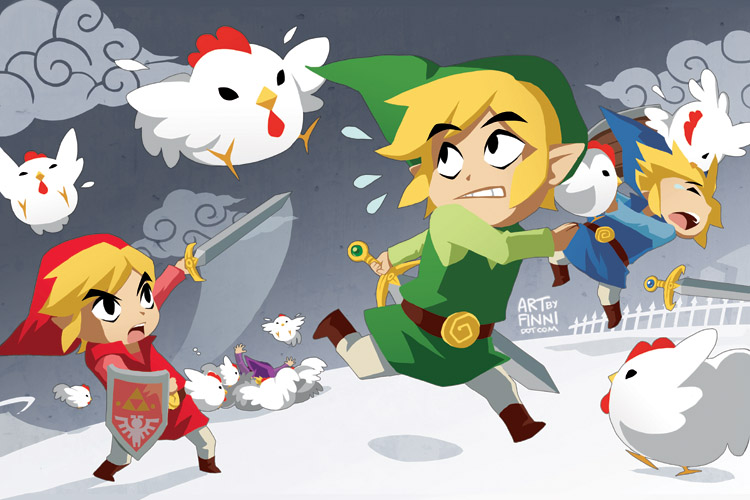
\includegraphics[width=0.7\textwidth]{figures/Sample/tumblr_static_eaceks0rfxsss8o4swscw40wo.jpg}
		\caption{Figure 2}
		\label{fig_multienv_2}
	\end{subfigure}
	
	\caption{A Multi-Figure Environment}
	\label{fig_multienv}
\end{figure}

\section{Tables}

Here is a sample table (Table~\ref{tab_sample}):

	\begin{table}[ht]
	\centering
	\begin{tabular}{ m{0.2\textwidth} m {0.1\textwidth} m{0.15\textwidth} }
		\toprule
		A & $\longleftrightarrow$ & B \\
		C & $\longleftrightarrow$ & D \\
		\bottomrule	
	\end{tabular}	
	\caption{A sample table}	
	\label{tab_sample}
\end{table}

\subsection{Long Tables}
A sample long table is shown in Appendix~\ref{appendix_b}.

\section{Equations}

Here is a sample equation (Equation~\ref{eq_lineslope}):

\begin{equation} \label{eq_lineslope}
	y = mx + b
=======
\chapter{Your Chapter Title}

This is a sample chapter

If you need to use quotes, type it ``like this''.

\section{Referencing}
These are some sample references to GAMYGDALA~\citep{popescu2014gamygdala} from 
the \texttt{references.bib} file and state effects of 
cognition~\citep{hudlicka2002time} from the \texttt{references\_another.bib} 
file. These references are not in the same .bib file.

\section{Figures}
This is a single image figure (Figure~\ref{fig_singleenv}):

\begin{figure}[ht]
    \centering
    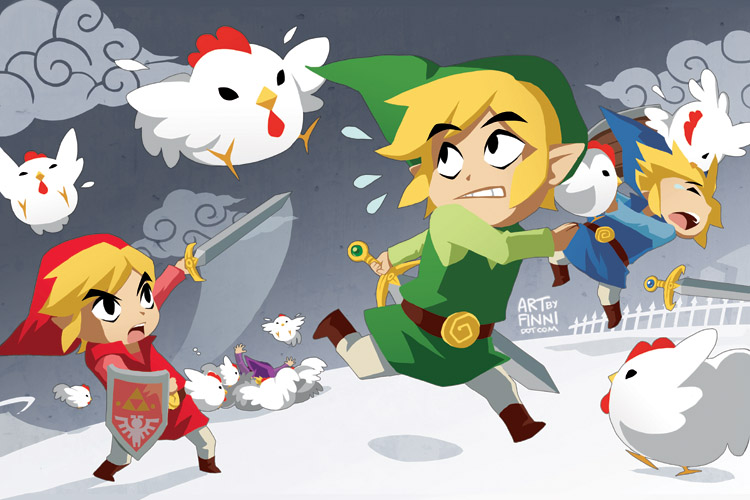
\includegraphics[width=0.6\textwidth]{figures/Sample/tumblr_static_eaceks0rfxsss8o4swscw40wo.jpg}
    \caption[Single Figure Environment Listed Title]{This is a single figure 
    environment}
    \label{fig_singleenv}
\end{figure}

This is a multi-image figure with a top (Figure~\ref{fig_multienv_1}) and bottom (Figure~\ref{fig_multienv_2}) aligned subfigures:

\begin{figure}[ht]
	\centering
	\begin{subfigure}[t]{\textwidth}
		\centering
		
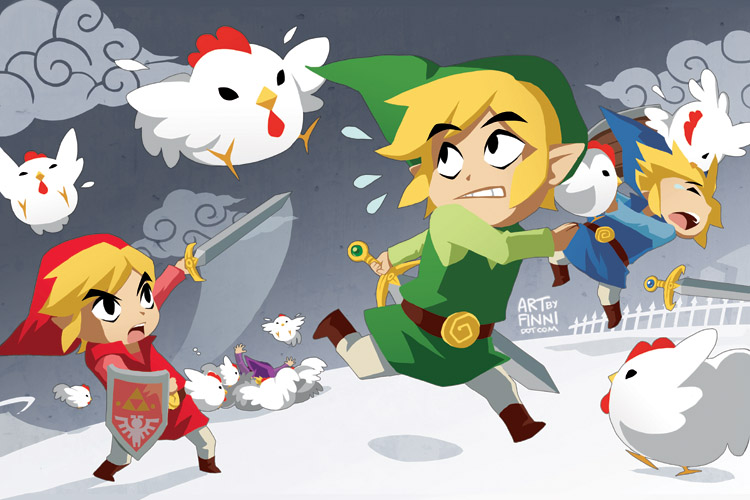
\includegraphics[width=0.7\textwidth]{figures/Sample/tumblr_static_eaceks0rfxsss8o4swscw40wo.jpg}
		\caption{Figure 1}
		\label{fig_multienv_1}
	\end{subfigure}
	~
	\begin{subfigure}[t]{\textwidth}
		\centering
		
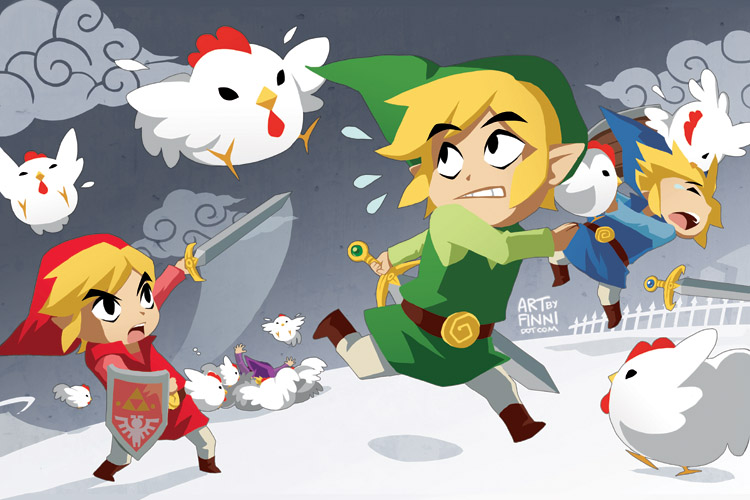
\includegraphics[width=0.7\textwidth]{figures/Sample/tumblr_static_eaceks0rfxsss8o4swscw40wo.jpg}
		\caption{Figure 2}
		\label{fig_multienv_2}
	\end{subfigure}
	
	\caption{A Multi-Figure Environment}
	\label{fig_multienv}
\end{figure}

\section{Tables}

Here is a sample table (Table~\ref{tab_sample}):

	\begin{table}[ht]
	\centering
	\begin{tabular}{ m{0.2\textwidth} m {0.1\textwidth} m{0.15\textwidth} }
		\toprule
		A & $\longleftrightarrow$ & B \\
		C & $\longleftrightarrow$ & D \\
		\bottomrule	
	\end{tabular}	
	\caption{A sample table}	
	\label{tab_sample}
\end{table}

\subsection{Long Tables}
A sample long table is shown in Appendix~\ref{appendix_b}.

\section{Equations}

Here is a sample equation (Equation~\ref{eq_lineslope}):

\begin{equation} \label{eq_lineslope}
	y = mx + b
>>>>>>> 9d845fd9678a4217417e588c8e1f2a2f78b24c2f
>>>>>>> Stashed changes
\end{equation}                  
       \setcounter{figure}{0}
       \setcounter{equation}{0}
       \setcounter{table}{0}

  <<<<<<< Updated upstream
\chapter{Conclusion}

=======
<<<<<<< HEAD
\chapter{Conclusion}

=======
\chapter{Conclusion}

>>>>>>> 9d845fd9678a4217417e588c8e1f2a2f78b24c2f
>>>>>>> Stashed changes
Every thesis also needs a concluding chapter
        \setcounter{figure}{0}
        \setcounter{equation}{0}
        \setcounter{table}{0}

\begin{appendix}
    <<<<<<< Updated upstream
\chapter{Your Appendix}
\label{appendix_a}

Your appendix goes here.
=======
<<<<<<< HEAD
\chapter{Your Appendix}
\label{appendix_a}

Your appendix goes here.
=======
\chapter{Your Appendix}
\label{appendix_a}

Your appendix goes here.
>>>>>>> 9d845fd9678a4217417e588c8e1f2a2f78b24c2f
>>>>>>> Stashed changes

        \setcounter{figure}{0}
        \setcounter{equation}{0}
        \setcounter{table}{0}

    <<<<<<< Updated upstream
\chapter{Long Tables}
\label{appendix_b}

This appendix demonstrates the use of a long table that spans multiple pages.

\begin{center}
\begin{longtable}{P{3cm}P{3cm}P{2.5cm}P{3.5cm}}
\toprule
\hline
\textbf{Col A} & \textbf{Col B} & \textbf{Col C} & \textbf{Col D} \\ \midrule

\endfirsthead
\multicolumn{4}{c}{\textit{Continued from previous page}} \\ \hline
\textbf{Col A} & \textbf{Col B} & \textbf{Col C} & \textbf{Col D} \\ \hline
\endhead
\hline \multicolumn{4}{r}{\textit{Continued on the next page}} \\
\endfoot
\hline
\endlastfoot

A & B & C & D \\ \midrule

A & B & C & D \\ \midrule

A & B & C & D \\ \midrule

A & B & C & D \\ \midrule

A & B & C & D \\ \midrule

A & B & C & D \\ \midrule

A & B & C & D \\ \midrule

A & B & C & D \\ \midrule

A & B & C & D \\ \midrule

A & B & C & D \\ \midrule

A & B & C & D \\ \midrule

A & B & C & D \\ \midrule

A & B & C & D \\ \midrule

A & B & C & D \\ \midrule

A & B & C & D \\ \midrule

A & B & C & D \\ \midrule

A & B & C & D \\ \midrule

A & B & C & D \\ \midrule

A & B & C & D \\ \midrule

A & B & C & D \\ \midrule

\hline
\end{longtable}
\end{center}
=======
<<<<<<< HEAD
\chapter{Long Tables}
\label{appendix_b}

This appendix demonstrates the use of a long table that spans multiple pages.

\begin{center}
\begin{longtable}{P{3cm}P{3cm}P{2.5cm}P{3.5cm}}
\toprule
\hline
\textbf{Col A} & \textbf{Col B} & \textbf{Col C} & \textbf{Col D} \\ \midrule

\endfirsthead
\multicolumn{4}{c}{\textit{Continued from previous page}} \\ \hline
\textbf{Col A} & \textbf{Col B} & \textbf{Col C} & \textbf{Col D} \\ \hline
\endhead
\hline \multicolumn{4}{r}{\textit{Continued on the next page}} \\
\endfoot
\hline
\endlastfoot

A & B & C & D \\ \midrule

A & B & C & D \\ \midrule

A & B & C & D \\ \midrule

A & B & C & D \\ \midrule

A & B & C & D \\ \midrule

A & B & C & D \\ \midrule

A & B & C & D \\ \midrule

A & B & C & D \\ \midrule

A & B & C & D \\ \midrule

A & B & C & D \\ \midrule

A & B & C & D \\ \midrule

A & B & C & D \\ \midrule

A & B & C & D \\ \midrule

A & B & C & D \\ \midrule

A & B & C & D \\ \midrule

A & B & C & D \\ \midrule

A & B & C & D \\ \midrule

A & B & C & D \\ \midrule

A & B & C & D \\ \midrule

A & B & C & D \\ \midrule

\hline
\end{longtable}
\end{center}
=======
\chapter{Long Tables}
\label{appendix_b}

This appendix demonstrates the use of a long table that spans multiple pages.

\begin{center}
\begin{longtable}{P{3cm}P{3cm}P{2.5cm}P{3.5cm}}
\toprule
\hline
\textbf{Col A} & \textbf{Col B} & \textbf{Col C} & \textbf{Col D} \\ \midrule

\endfirsthead
\multicolumn{4}{c}{\textit{Continued from previous page}} \\ \hline
\textbf{Col A} & \textbf{Col B} & \textbf{Col C} & \textbf{Col D} \\ \hline
\endhead
\hline \multicolumn{4}{r}{\textit{Continued on the next page}} \\
\endfoot
\hline
\endlastfoot

A & B & C & D \\ \midrule

A & B & C & D \\ \midrule

A & B & C & D \\ \midrule

A & B & C & D \\ \midrule

A & B & C & D \\ \midrule

A & B & C & D \\ \midrule

A & B & C & D \\ \midrule

A & B & C & D \\ \midrule

A & B & C & D \\ \midrule

A & B & C & D \\ \midrule

A & B & C & D \\ \midrule

A & B & C & D \\ \midrule

A & B & C & D \\ \midrule

A & B & C & D \\ \midrule

A & B & C & D \\ \midrule

A & B & C & D \\ \midrule

A & B & C & D \\ \midrule

A & B & C & D \\ \midrule

A & B & C & D \\ \midrule

A & B & C & D \\ \midrule

\hline
\end{longtable}
\end{center}
>>>>>>> 9d845fd9678a4217417e588c8e1f2a2f78b24c2f
>>>>>>> Stashed changes

        \setcounter{figure}{0}
        \setcounter{equation}{0}
        \setcounter{table}{0}
\end{appendix}

% The bibliography is set up to allow for multiple bib files
\bibliographystyle{ACM-Reference-Format}
\bibliography{references,references_another}

\label{NumDocumentPages}

\end{document}
% ********************************
=======
<<<<<<< HEAD
\documentclass[12pt]{report} % Times New Roman, 12pt
%\usepackage{gscale_thesis_singlespace} % Single spaced thesis
\usepackage{gscale_thesis_doublespace} % Double spaced thesis
\usepackage{fancyheadings} % Header and footer styling
\usepackage{natbib} % Bibliography formatting
\usepackage{setspace} % Allows double spacing but skips headers/footers
\setcounter{tocdepth}{1} % Limits the TOC to chapter and section names

% Additional packages
\usepackage{graphicx} % Allows the inclusion of figures
\usepackage{subcaption} % Allows captions to be added to subfigures
\usepackage[justification=centering]{caption} % Centres caption text
\usepackage{array} % Used for table formatting
\newcolumntype{P}[1]{>{\raggedright\let\newline\\\arraybackslash\hspace{0pt}}m{#1}}
\usepackage{booktabs} % Fancy-style tables
\usepackage{longtable} % Allows for tables that are more than one page long
\usepackage{float} % Better figure placement control
\usepackage{enumerate} % Numbered lists
\usepackage[shortlabels]{enumitem} % For controlling enumerate labels
\usepackage[shortcuts]{extdash} % Allows manual hyphenation of hypenated words
\usepackage{amsmath} % Non-standard math symbols
\usepackage{amsfonts} % Extended fonts for mathematics

\usepackage[hidelinks]{hyperref} % Linking to LaTeX labels and external URLs

\numberwithin{equation}{section} % Numbers equations based on their section

% ********************************
\begin{document}
<<<<<<< Updated upstream
\title{Your Thesis Title, Which Can Be As Long As You Want On the Title Page}
\halftitle{Short Title} % 60 Characters Max. Including Spaces

\author{Jane Doe}
\shortauthor{J. Doe} % Used for page header

\dept{Department You Belong To}
\field{Your Field} % What field your thesis is in (e.g. Software Engineering)

\prevdegreeone{B.Eng. (Software Engineering \& Game Design),\\ McMaster University, Hamilton, Canada}
\prevdegreetwo{B.Eng.} % Just your degree's field

\submitdate{MONTH YEAR} % Use the month's full spelling e.g. November
\copyrightyear{YYYY} % Year you are submitting this, usually your graduation 
%year

\doctype{Report} % ``Report'' or ``Thesis'' or whatever you need
\degree{Masters of Engineering} % The degree you get when you submit this
\degreeabbrv{M.Eng.}
\principaladviser{Your Supervisor} % Your Supervisor
=======
<<<<<<< HEAD
\title{Your Thesis Title, Which Can Be As Long As You Want On the Title Page}
\halftitle{Short Title} % 60 Characters Max. Including Spaces

\author{Jane Doe}
\shortauthor{J. Doe} % Used for page header

\dept{Department You Belong To}
\field{Your Field} % What field your thesis is in (e.g. Software Engineering)

\prevdegreeone{B.Eng. (Software Engineering \& Game Design),\\ McMaster University, Hamilton, Canada}
\prevdegreetwo{B.Eng.} % Just your degree's field

\submitdate{MONTH YEAR} % Use the month's full spelling e.g. November
\copyrightyear{YYYY} % Year you are submitting this, usually your graduation 
%year

\doctype{Report} % ``Report'' or ``Thesis'' or whatever you need
\degree{Masters of Engineering} % The degree you get when you submit this
\degreeabbrv{M.Eng.}
\principaladviser{Your Supervisor} % Your Supervisor
=======
\title{Your Thesis Title, Which Can Be As Long As You Want On the Title Page}
\halftitle{Short Title} % 60 Characters Max. Including Spaces

\author{Jane Doe}
\shortauthor{J. Doe} % Used for page header

\dept{Department You Belong To}
\field{Your Field} % What field your thesis is in (e.g. Software Engineering)

\prevdegreeone{B.Eng. (Software Engineering \& Game Design),\\ McMaster University, Hamilton, Canada}
\prevdegreetwo{B.Eng.} % Just your degree's field

\submitdate{MONTH YEAR} % Use the month's full spelling e.g. November
\copyrightyear{YYYY} % Year you are submitting this, usually your graduation 
%year

\doctype{Report} % ``Report'' or ``Thesis'' or whatever you need
\degree{Masters of Engineering} % The degree you get when you submit this
\degreeabbrv{M.Eng.}
\principaladviser{Your Supervisor} % Your Supervisor
>>>>>>> 9d845fd9678a4217417e588c8e1f2a2f78b24c2f
>>>>>>> Stashed changes
 % LaTeX variables for preface pages/headers
    
\beforepreface % Half title page, title page, declaration page   
  <<<<<<< Updated upstream
\prefacesection{Lay Abstract}

=======
<<<<<<< HEAD
\prefacesection{Lay Abstract}

=======
\prefacesection{Lay Abstract}

>>>>>>> 9d845fd9678a4217417e588c8e1f2a2f78b24c2f
>>>>>>> Stashed changes
A lay abstract of not more 150 words must be included explaining the key goals and contributions of the thesis in lay terms that is accessible to the general public.  % Lay Abstract
  <<<<<<< Updated upstream
\prefacesection{Abstract}

=======
<<<<<<< HEAD
\prefacesection{Abstract}

=======
\prefacesection{Abstract}

>>>>>>> 9d845fd9678a4217417e588c8e1f2a2f78b24c2f
>>>>>>> Stashed changes
Abstract here (no more than 300 words) % Abstract
  <<<<<<< Updated upstream
%\thispagestyle{empty}
\null\vfill
\begin{center}
%\textbf{Dedications}
%\linebreak
\textsl{Your Dedication \\ Optional second line}
\end{center}
\vfill
=======
<<<<<<< HEAD
%\thispagestyle{empty}
\null\vfill
\begin{center}
%\textbf{Dedications}
%\linebreak
\textsl{Your Dedication \\ Optional second line}
\end{center}
\vfill
=======
%\thispagestyle{empty}
\null\vfill
\begin{center}
%\textbf{Dedications}
%\linebreak
\textsl{Your Dedication \\ Optional second line}
\end{center}
\vfill
>>>>>>> 9d845fd9678a4217417e588c8e1f2a2f78b24c2f
>>>>>>> Stashed changes
 % Dedication
  <<<<<<< Updated upstream
\prefacesection{Acknowledgements}

=======
<<<<<<< HEAD
\prefacesection{Acknowledgements}

=======
\prefacesection{Acknowledgements}

>>>>>>> 9d845fd9678a4217417e588c8e1f2a2f78b24c2f
>>>>>>> Stashed changes
Acknowledgements go here. % Acknowledgements
  \referencepages % Table of Contents, List of Figures, List of Tables
  <<<<<<< Updated upstream
\prefacesection{Notation, Definitions, and Abbreviations}

\section*{Notation}
\begin{description}[font=\rmfamily\bfseries, leftmargin=3cm, style=nextline]
	\item[$A \leq B$] A is less than or equal to B
\end{description}

\section*{Definitions}
\begin{description}[font=\rmfamily\bfseries, leftmargin=3cm, style=nextline]
	\item[Challenge] With respect to video games, a challenge is a set of goals presented to the player that they are tasks with completing; challenges can test a variety of player skills, including accuracy, logical reasoning, and creative problem solving
\end{description}

\section*{Abbreviations}
\begin{description}[font=\rmfamily\bfseries, leftmargin=3cm, style=nextline]
	\item[AI] Artificial intelligence
=======
<<<<<<< HEAD
\prefacesection{Notation, Definitions, and Abbreviations}

\section*{Notation}
\begin{description}[font=\rmfamily\bfseries, leftmargin=3cm, style=nextline]
	\item[$A \leq B$] A is less than or equal to B
\end{description}

\section*{Definitions}
\begin{description}[font=\rmfamily\bfseries, leftmargin=3cm, style=nextline]
	\item[Challenge] With respect to video games, a challenge is a set of goals presented to the player that they are tasks with completing; challenges can test a variety of player skills, including accuracy, logical reasoning, and creative problem solving
\end{description}

\section*{Abbreviations}
\begin{description}[font=\rmfamily\bfseries, leftmargin=3cm, style=nextline]
	\item[AI] Artificial intelligence
=======
\prefacesection{Notation, Definitions, and Abbreviations}

\section*{Notation}
\begin{description}[font=\rmfamily\bfseries, leftmargin=3cm, style=nextline]
	\item[$A \leq B$] A is less than or equal to B
\end{description}

\section*{Definitions}
\begin{description}[font=\rmfamily\bfseries, leftmargin=3cm, style=nextline]
	\item[Challenge] With respect to video games, a challenge is a set of goals presented to the player that they are tasks with completing; challenges can test a variety of player skills, including accuracy, logical reasoning, and creative problem solving
\end{description}

\section*{Abbreviations}
\begin{description}[font=\rmfamily\bfseries, leftmargin=3cm, style=nextline]
	\item[AI] Artificial intelligence
>>>>>>> 9d845fd9678a4217417e588c8e1f2a2f78b24c2f
>>>>>>> Stashed changes
\end{description}
  \academicstatement{academicachievementdeclaration}
\afterpreface
  
  
  <<<<<<< Updated upstream
\chapter{Introduction}

Every thesis needs an introductory chapter

While you're here, you need to go into \texttt{definitions.tex} to set all the 
information needed for the front matter (e.g. title, author) and page 
header/footer.

You will also find the School of Graduate Studies' preparation guide (August 
2021) for theses and reports. I would give it a quick read so you know what's 
=======
<<<<<<< HEAD
\chapter{Introduction}

Every thesis needs an introductory chapter

While you're here, you need to go into \texttt{definitions.tex} to set all the 
information needed for the front matter (e.g. title, author) and page 
header/footer.

You will also find the School of Graduate Studies' preparation guide (August 
2021) for theses and reports. I would give it a quick read so you know what's 
=======
\chapter{Introduction}

Every thesis needs an introductory chapter

While you're here, you need to go into \texttt{definitions.tex} to set all the 
information needed for the front matter (e.g. title, author) and page 
header/footer.

You will also find the School of Graduate Studies' preparation guide (August 
2021) for theses and reports. I would give it a quick read so you know what's 
>>>>>>> 9d845fd9678a4217417e588c8e1f2a2f78b24c2f
>>>>>>> Stashed changes
expected.                  
        \setcounter{figure}{0}
        \setcounter{equation}{0}
        \setcounter{table}{0}
        
  <<<<<<< Updated upstream
\chapter{Your Chapter Title}

This is a sample chapter

If you need to use quotes, type it ``like this''.

\section{Referencing}
These are some sample references to GAMYGDALA~\citep{popescu2014gamygdala} from 
the \texttt{references.bib} file and state effects of 
cognition~\citep{hudlicka2002time} from the \texttt{references\_another.bib} 
file. These references are not in the same .bib file.

\section{Figures}
This is a single image figure (Figure~\ref{fig_singleenv}):

\begin{figure}[ht]
    \centering
    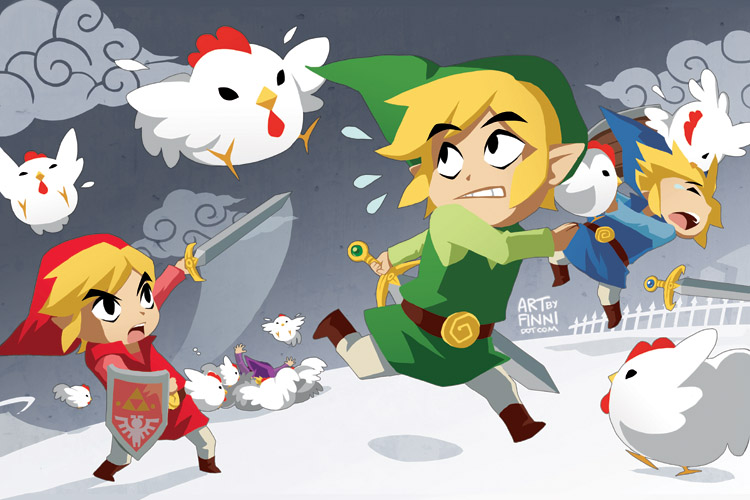
\includegraphics[width=0.6\textwidth]{figures/Sample/tumblr_static_eaceks0rfxsss8o4swscw40wo.jpg}
    \caption[Single Figure Environment Listed Title]{This is a single figure 
    environment}
    \label{fig_singleenv}
\end{figure}

This is a multi-image figure with a top (Figure~\ref{fig_multienv_1}) and bottom (Figure~\ref{fig_multienv_2}) aligned subfigures:

\begin{figure}[ht]
	\centering
	\begin{subfigure}[t]{\textwidth}
		\centering
		
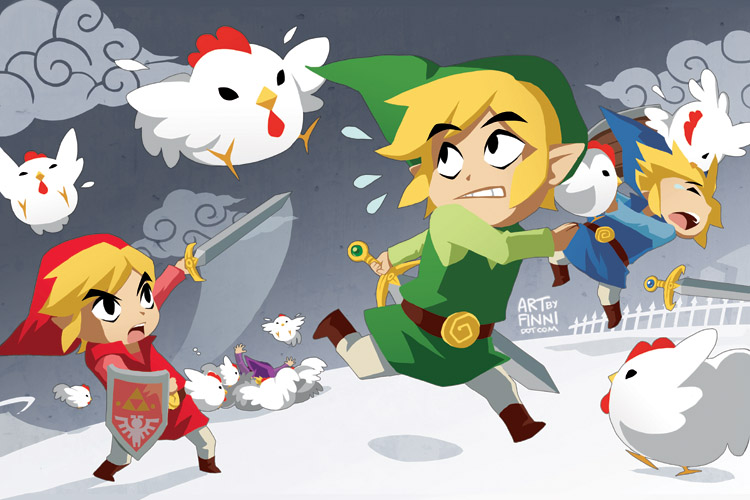
\includegraphics[width=0.7\textwidth]{figures/Sample/tumblr_static_eaceks0rfxsss8o4swscw40wo.jpg}
		\caption{Figure 1}
		\label{fig_multienv_1}
	\end{subfigure}
	~
	\begin{subfigure}[t]{\textwidth}
		\centering
		
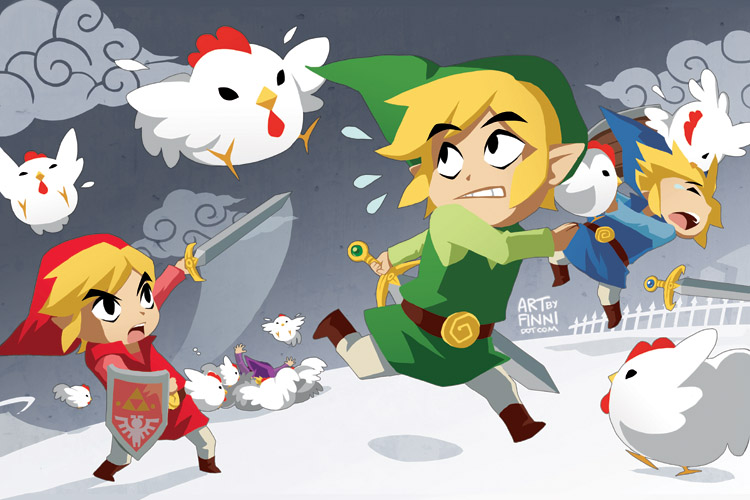
\includegraphics[width=0.7\textwidth]{figures/Sample/tumblr_static_eaceks0rfxsss8o4swscw40wo.jpg}
		\caption{Figure 2}
		\label{fig_multienv_2}
	\end{subfigure}
	
	\caption{A Multi-Figure Environment}
	\label{fig_multienv}
\end{figure}

\section{Tables}

Here is a sample table (Table~\ref{tab_sample}):

	\begin{table}[ht]
	\centering
	\begin{tabular}{ m{0.2\textwidth} m {0.1\textwidth} m{0.15\textwidth} }
		\toprule
		A & $\longleftrightarrow$ & B \\
		C & $\longleftrightarrow$ & D \\
		\bottomrule	
	\end{tabular}	
	\caption{A sample table}	
	\label{tab_sample}
\end{table}

\subsection{Long Tables}
A sample long table is shown in Appendix~\ref{appendix_b}.

\section{Equations}

Here is a sample equation (Equation~\ref{eq_lineslope}):

\begin{equation} \label{eq_lineslope}
	y = mx + b
=======
<<<<<<< HEAD
\chapter{Your Chapter Title}

This is a sample chapter

If you need to use quotes, type it ``like this''.

\section{Referencing}
These are some sample references to GAMYGDALA~\citep{popescu2014gamygdala} from 
the \texttt{references.bib} file and state effects of 
cognition~\citep{hudlicka2002time} from the \texttt{references\_another.bib} 
file. These references are not in the same .bib file.

\section{Figures}
This is a single image figure (Figure~\ref{fig_singleenv}):

\begin{figure}[ht]
    \centering
    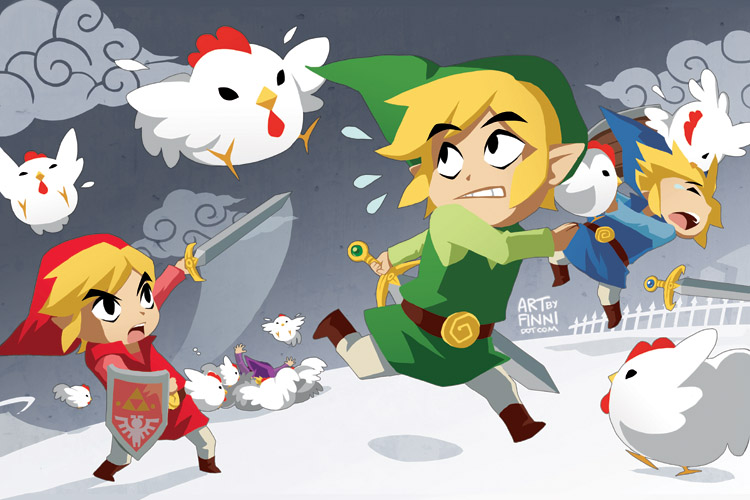
\includegraphics[width=0.6\textwidth]{figures/Sample/tumblr_static_eaceks0rfxsss8o4swscw40wo.jpg}
    \caption[Single Figure Environment Listed Title]{This is a single figure 
    environment}
    \label{fig_singleenv}
\end{figure}

This is a multi-image figure with a top (Figure~\ref{fig_multienv_1}) and bottom (Figure~\ref{fig_multienv_2}) aligned subfigures:

\begin{figure}[ht]
	\centering
	\begin{subfigure}[t]{\textwidth}
		\centering
		
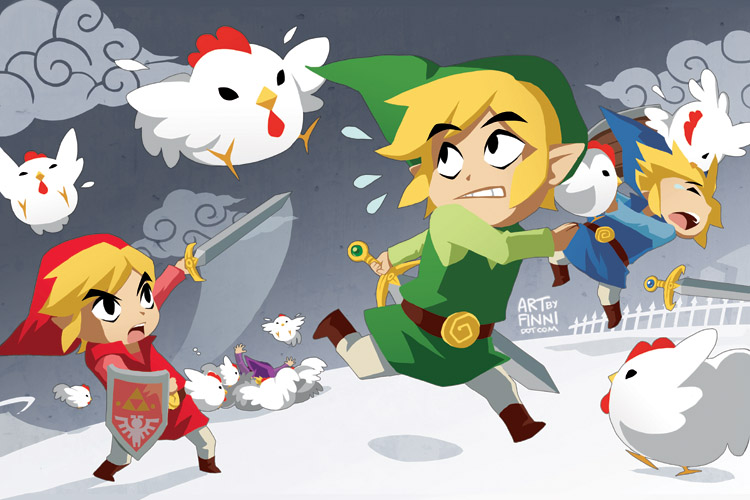
\includegraphics[width=0.7\textwidth]{figures/Sample/tumblr_static_eaceks0rfxsss8o4swscw40wo.jpg}
		\caption{Figure 1}
		\label{fig_multienv_1}
	\end{subfigure}
	~
	\begin{subfigure}[t]{\textwidth}
		\centering
		
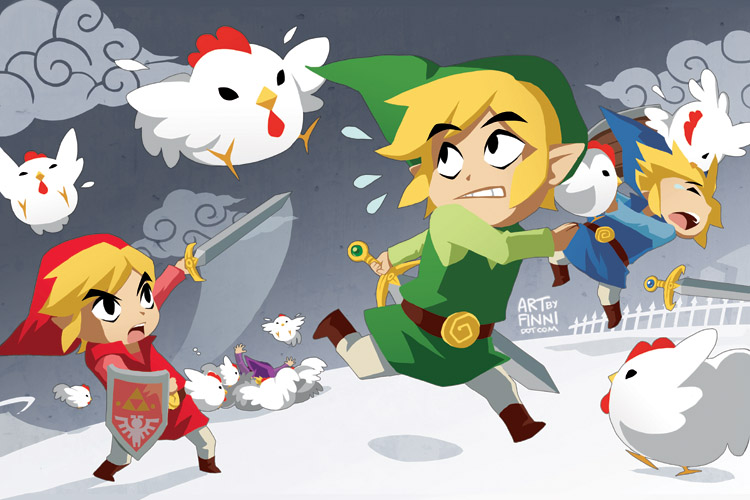
\includegraphics[width=0.7\textwidth]{figures/Sample/tumblr_static_eaceks0rfxsss8o4swscw40wo.jpg}
		\caption{Figure 2}
		\label{fig_multienv_2}
	\end{subfigure}
	
	\caption{A Multi-Figure Environment}
	\label{fig_multienv}
\end{figure}

\section{Tables}

Here is a sample table (Table~\ref{tab_sample}):

	\begin{table}[ht]
	\centering
	\begin{tabular}{ m{0.2\textwidth} m {0.1\textwidth} m{0.15\textwidth} }
		\toprule
		A & $\longleftrightarrow$ & B \\
		C & $\longleftrightarrow$ & D \\
		\bottomrule	
	\end{tabular}	
	\caption{A sample table}	
	\label{tab_sample}
\end{table}

\subsection{Long Tables}
A sample long table is shown in Appendix~\ref{appendix_b}.

\section{Equations}

Here is a sample equation (Equation~\ref{eq_lineslope}):

\begin{equation} \label{eq_lineslope}
	y = mx + b
=======
\chapter{Your Chapter Title}

This is a sample chapter

If you need to use quotes, type it ``like this''.

\section{Referencing}
These are some sample references to GAMYGDALA~\citep{popescu2014gamygdala} from 
the \texttt{references.bib} file and state effects of 
cognition~\citep{hudlicka2002time} from the \texttt{references\_another.bib} 
file. These references are not in the same .bib file.

\section{Figures}
This is a single image figure (Figure~\ref{fig_singleenv}):

\begin{figure}[ht]
    \centering
    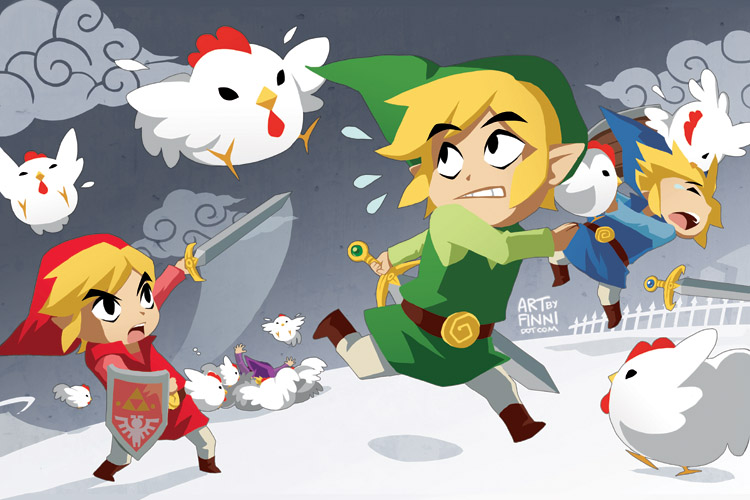
\includegraphics[width=0.6\textwidth]{figures/Sample/tumblr_static_eaceks0rfxsss8o4swscw40wo.jpg}
    \caption[Single Figure Environment Listed Title]{This is a single figure 
    environment}
    \label{fig_singleenv}
\end{figure}

This is a multi-image figure with a top (Figure~\ref{fig_multienv_1}) and bottom (Figure~\ref{fig_multienv_2}) aligned subfigures:

\begin{figure}[ht]
	\centering
	\begin{subfigure}[t]{\textwidth}
		\centering
		
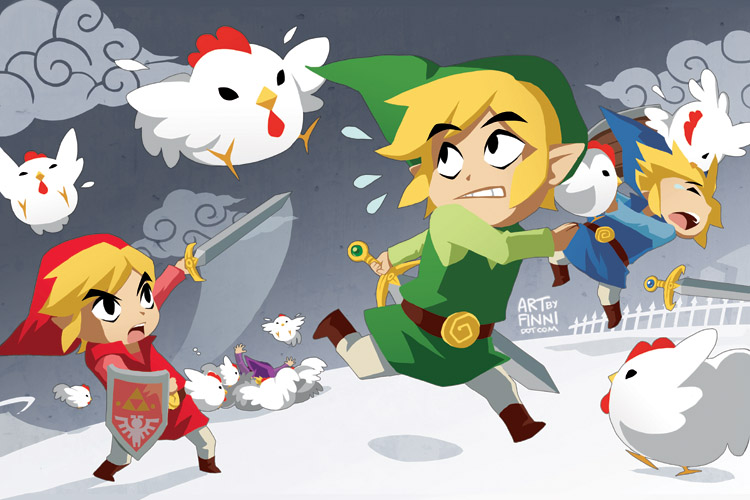
\includegraphics[width=0.7\textwidth]{figures/Sample/tumblr_static_eaceks0rfxsss8o4swscw40wo.jpg}
		\caption{Figure 1}
		\label{fig_multienv_1}
	\end{subfigure}
	~
	\begin{subfigure}[t]{\textwidth}
		\centering
		
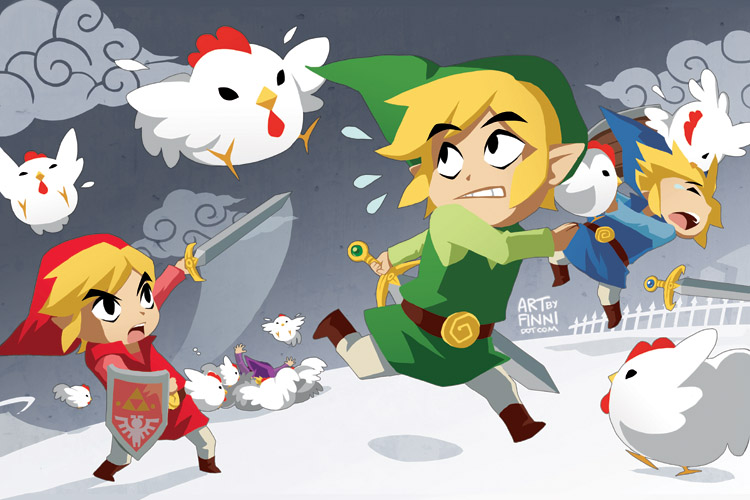
\includegraphics[width=0.7\textwidth]{figures/Sample/tumblr_static_eaceks0rfxsss8o4swscw40wo.jpg}
		\caption{Figure 2}
		\label{fig_multienv_2}
	\end{subfigure}
	
	\caption{A Multi-Figure Environment}
	\label{fig_multienv}
\end{figure}

\section{Tables}

Here is a sample table (Table~\ref{tab_sample}):

	\begin{table}[ht]
	\centering
	\begin{tabular}{ m{0.2\textwidth} m {0.1\textwidth} m{0.15\textwidth} }
		\toprule
		A & $\longleftrightarrow$ & B \\
		C & $\longleftrightarrow$ & D \\
		\bottomrule	
	\end{tabular}	
	\caption{A sample table}	
	\label{tab_sample}
\end{table}

\subsection{Long Tables}
A sample long table is shown in Appendix~\ref{appendix_b}.

\section{Equations}

Here is a sample equation (Equation~\ref{eq_lineslope}):

\begin{equation} \label{eq_lineslope}
	y = mx + b
>>>>>>> 9d845fd9678a4217417e588c8e1f2a2f78b24c2f
>>>>>>> Stashed changes
\end{equation}                  
       \setcounter{figure}{0}
       \setcounter{equation}{0}
       \setcounter{table}{0}

  <<<<<<< Updated upstream
\chapter{Conclusion}

=======
<<<<<<< HEAD
\chapter{Conclusion}

=======
\chapter{Conclusion}

>>>>>>> 9d845fd9678a4217417e588c8e1f2a2f78b24c2f
>>>>>>> Stashed changes
Every thesis also needs a concluding chapter
        \setcounter{figure}{0}
        \setcounter{equation}{0}
        \setcounter{table}{0}

\begin{appendix}
    <<<<<<< Updated upstream
\chapter{Your Appendix}
\label{appendix_a}

Your appendix goes here.
=======
<<<<<<< HEAD
\chapter{Your Appendix}
\label{appendix_a}

Your appendix goes here.
=======
\chapter{Your Appendix}
\label{appendix_a}

Your appendix goes here.
>>>>>>> 9d845fd9678a4217417e588c8e1f2a2f78b24c2f
>>>>>>> Stashed changes

        \setcounter{figure}{0}
        \setcounter{equation}{0}
        \setcounter{table}{0}

    <<<<<<< Updated upstream
\chapter{Long Tables}
\label{appendix_b}

This appendix demonstrates the use of a long table that spans multiple pages.

\begin{center}
\begin{longtable}{P{3cm}P{3cm}P{2.5cm}P{3.5cm}}
\toprule
\hline
\textbf{Col A} & \textbf{Col B} & \textbf{Col C} & \textbf{Col D} \\ \midrule

\endfirsthead
\multicolumn{4}{c}{\textit{Continued from previous page}} \\ \hline
\textbf{Col A} & \textbf{Col B} & \textbf{Col C} & \textbf{Col D} \\ \hline
\endhead
\hline \multicolumn{4}{r}{\textit{Continued on the next page}} \\
\endfoot
\hline
\endlastfoot

A & B & C & D \\ \midrule

A & B & C & D \\ \midrule

A & B & C & D \\ \midrule

A & B & C & D \\ \midrule

A & B & C & D \\ \midrule

A & B & C & D \\ \midrule

A & B & C & D \\ \midrule

A & B & C & D \\ \midrule

A & B & C & D \\ \midrule

A & B & C & D \\ \midrule

A & B & C & D \\ \midrule

A & B & C & D \\ \midrule

A & B & C & D \\ \midrule

A & B & C & D \\ \midrule

A & B & C & D \\ \midrule

A & B & C & D \\ \midrule

A & B & C & D \\ \midrule

A & B & C & D \\ \midrule

A & B & C & D \\ \midrule

A & B & C & D \\ \midrule

\hline
\end{longtable}
\end{center}
=======
<<<<<<< HEAD
\chapter{Long Tables}
\label{appendix_b}

This appendix demonstrates the use of a long table that spans multiple pages.

\begin{center}
\begin{longtable}{P{3cm}P{3cm}P{2.5cm}P{3.5cm}}
\toprule
\hline
\textbf{Col A} & \textbf{Col B} & \textbf{Col C} & \textbf{Col D} \\ \midrule

\endfirsthead
\multicolumn{4}{c}{\textit{Continued from previous page}} \\ \hline
\textbf{Col A} & \textbf{Col B} & \textbf{Col C} & \textbf{Col D} \\ \hline
\endhead
\hline \multicolumn{4}{r}{\textit{Continued on the next page}} \\
\endfoot
\hline
\endlastfoot

A & B & C & D \\ \midrule

A & B & C & D \\ \midrule

A & B & C & D \\ \midrule

A & B & C & D \\ \midrule

A & B & C & D \\ \midrule

A & B & C & D \\ \midrule

A & B & C & D \\ \midrule

A & B & C & D \\ \midrule

A & B & C & D \\ \midrule

A & B & C & D \\ \midrule

A & B & C & D \\ \midrule

A & B & C & D \\ \midrule

A & B & C & D \\ \midrule

A & B & C & D \\ \midrule

A & B & C & D \\ \midrule

A & B & C & D \\ \midrule

A & B & C & D \\ \midrule

A & B & C & D \\ \midrule

A & B & C & D \\ \midrule

A & B & C & D \\ \midrule

\hline
\end{longtable}
\end{center}
=======
\chapter{Long Tables}
\label{appendix_b}

This appendix demonstrates the use of a long table that spans multiple pages.

\begin{center}
\begin{longtable}{P{3cm}P{3cm}P{2.5cm}P{3.5cm}}
\toprule
\hline
\textbf{Col A} & \textbf{Col B} & \textbf{Col C} & \textbf{Col D} \\ \midrule

\endfirsthead
\multicolumn{4}{c}{\textit{Continued from previous page}} \\ \hline
\textbf{Col A} & \textbf{Col B} & \textbf{Col C} & \textbf{Col D} \\ \hline
\endhead
\hline \multicolumn{4}{r}{\textit{Continued on the next page}} \\
\endfoot
\hline
\endlastfoot

A & B & C & D \\ \midrule

A & B & C & D \\ \midrule

A & B & C & D \\ \midrule

A & B & C & D \\ \midrule

A & B & C & D \\ \midrule

A & B & C & D \\ \midrule

A & B & C & D \\ \midrule

A & B & C & D \\ \midrule

A & B & C & D \\ \midrule

A & B & C & D \\ \midrule

A & B & C & D \\ \midrule

A & B & C & D \\ \midrule

A & B & C & D \\ \midrule

A & B & C & D \\ \midrule

A & B & C & D \\ \midrule

A & B & C & D \\ \midrule

A & B & C & D \\ \midrule

A & B & C & D \\ \midrule

A & B & C & D \\ \midrule

A & B & C & D \\ \midrule

\hline
\end{longtable}
\end{center}
>>>>>>> 9d845fd9678a4217417e588c8e1f2a2f78b24c2f
>>>>>>> Stashed changes

        \setcounter{figure}{0}
        \setcounter{equation}{0}
        \setcounter{table}{0}
\end{appendix}

% The bibliography is set up to allow for multiple bib files
\bibliographystyle{ACM-Reference-Format}
\bibliography{references,references_another}

\label{NumDocumentPages}

\end{document}
% ********************************
=======
\documentclass[12pt]{report} % Times New Roman, 12pt
%\usepackage{gscale_thesis_singlespace} % Single spaced thesis
\usepackage{gscale_thesis_doublespace} % Double spaced thesis
\usepackage{fancyheadings} % Header and footer styling
\usepackage{natbib} % Bibliography formatting
\usepackage{setspace} % Allows double spacing but skips headers/footers
\setcounter{tocdepth}{1} % Limits the TOC to chapter and section names

% Additional packages
\usepackage{graphicx} % Allows the inclusion of figures
\usepackage{subcaption} % Allows captions to be added to subfigures
\usepackage[justification=centering]{caption} % Centres caption text
\usepackage{array} % Used for table formatting
\newcolumntype{P}[1]{>{\raggedright\let\newline\\\arraybackslash\hspace{0pt}}m{#1}}
\usepackage{booktabs} % Fancy-style tables
\usepackage{longtable} % Allows for tables that are more than one page long
\usepackage{float} % Better figure placement control
\usepackage{enumerate} % Numbered lists
\usepackage[shortlabels]{enumitem} % For controlling enumerate labels
\usepackage[shortcuts]{extdash} % Allows manual hyphenation of hypenated words
\usepackage{amsmath} % Non-standard math symbols
\usepackage{amsfonts} % Extended fonts for mathematics

\usepackage[hidelinks]{hyperref} % Linking to LaTeX labels and external URLs

\numberwithin{equation}{section} % Numbers equations based on their section

% ********************************
\begin{document}
<<<<<<< Updated upstream
\title{Your Thesis Title, Which Can Be As Long As You Want On the Title Page}
\halftitle{Short Title} % 60 Characters Max. Including Spaces

\author{Jane Doe}
\shortauthor{J. Doe} % Used for page header

\dept{Department You Belong To}
\field{Your Field} % What field your thesis is in (e.g. Software Engineering)

\prevdegreeone{B.Eng. (Software Engineering \& Game Design),\\ McMaster University, Hamilton, Canada}
\prevdegreetwo{B.Eng.} % Just your degree's field

\submitdate{MONTH YEAR} % Use the month's full spelling e.g. November
\copyrightyear{YYYY} % Year you are submitting this, usually your graduation 
%year

\doctype{Report} % ``Report'' or ``Thesis'' or whatever you need
\degree{Masters of Engineering} % The degree you get when you submit this
\degreeabbrv{M.Eng.}
\principaladviser{Your Supervisor} % Your Supervisor
=======
<<<<<<< HEAD
\title{Your Thesis Title, Which Can Be As Long As You Want On the Title Page}
\halftitle{Short Title} % 60 Characters Max. Including Spaces

\author{Jane Doe}
\shortauthor{J. Doe} % Used for page header

\dept{Department You Belong To}
\field{Your Field} % What field your thesis is in (e.g. Software Engineering)

\prevdegreeone{B.Eng. (Software Engineering \& Game Design),\\ McMaster University, Hamilton, Canada}
\prevdegreetwo{B.Eng.} % Just your degree's field

\submitdate{MONTH YEAR} % Use the month's full spelling e.g. November
\copyrightyear{YYYY} % Year you are submitting this, usually your graduation 
%year

\doctype{Report} % ``Report'' or ``Thesis'' or whatever you need
\degree{Masters of Engineering} % The degree you get when you submit this
\degreeabbrv{M.Eng.}
\principaladviser{Your Supervisor} % Your Supervisor
=======
\title{Your Thesis Title, Which Can Be As Long As You Want On the Title Page}
\halftitle{Short Title} % 60 Characters Max. Including Spaces

\author{Jane Doe}
\shortauthor{J. Doe} % Used for page header

\dept{Department You Belong To}
\field{Your Field} % What field your thesis is in (e.g. Software Engineering)

\prevdegreeone{B.Eng. (Software Engineering \& Game Design),\\ McMaster University, Hamilton, Canada}
\prevdegreetwo{B.Eng.} % Just your degree's field

\submitdate{MONTH YEAR} % Use the month's full spelling e.g. November
\copyrightyear{YYYY} % Year you are submitting this, usually your graduation 
%year

\doctype{Report} % ``Report'' or ``Thesis'' or whatever you need
\degree{Masters of Engineering} % The degree you get when you submit this
\degreeabbrv{M.Eng.}
\principaladviser{Your Supervisor} % Your Supervisor
>>>>>>> 9d845fd9678a4217417e588c8e1f2a2f78b24c2f
>>>>>>> Stashed changes
 % LaTeX variables for preface pages/headers
    
\beforepreface % Half title page, title page, declaration page   
  <<<<<<< Updated upstream
\prefacesection{Lay Abstract}

=======
<<<<<<< HEAD
\prefacesection{Lay Abstract}

=======
\prefacesection{Lay Abstract}

>>>>>>> 9d845fd9678a4217417e588c8e1f2a2f78b24c2f
>>>>>>> Stashed changes
A lay abstract of not more 150 words must be included explaining the key goals and contributions of the thesis in lay terms that is accessible to the general public.  % Lay Abstract
  <<<<<<< Updated upstream
\prefacesection{Abstract}

=======
<<<<<<< HEAD
\prefacesection{Abstract}

=======
\prefacesection{Abstract}

>>>>>>> 9d845fd9678a4217417e588c8e1f2a2f78b24c2f
>>>>>>> Stashed changes
Abstract here (no more than 300 words) % Abstract
  <<<<<<< Updated upstream
%\thispagestyle{empty}
\null\vfill
\begin{center}
%\textbf{Dedications}
%\linebreak
\textsl{Your Dedication \\ Optional second line}
\end{center}
\vfill
=======
<<<<<<< HEAD
%\thispagestyle{empty}
\null\vfill
\begin{center}
%\textbf{Dedications}
%\linebreak
\textsl{Your Dedication \\ Optional second line}
\end{center}
\vfill
=======
%\thispagestyle{empty}
\null\vfill
\begin{center}
%\textbf{Dedications}
%\linebreak
\textsl{Your Dedication \\ Optional second line}
\end{center}
\vfill
>>>>>>> 9d845fd9678a4217417e588c8e1f2a2f78b24c2f
>>>>>>> Stashed changes
 % Dedication
  <<<<<<< Updated upstream
\prefacesection{Acknowledgements}

=======
<<<<<<< HEAD
\prefacesection{Acknowledgements}

=======
\prefacesection{Acknowledgements}

>>>>>>> 9d845fd9678a4217417e588c8e1f2a2f78b24c2f
>>>>>>> Stashed changes
Acknowledgements go here. % Acknowledgements
  \referencepages % Table of Contents, List of Figures, List of Tables
  <<<<<<< Updated upstream
\prefacesection{Notation, Definitions, and Abbreviations}

\section*{Notation}
\begin{description}[font=\rmfamily\bfseries, leftmargin=3cm, style=nextline]
	\item[$A \leq B$] A is less than or equal to B
\end{description}

\section*{Definitions}
\begin{description}[font=\rmfamily\bfseries, leftmargin=3cm, style=nextline]
	\item[Challenge] With respect to video games, a challenge is a set of goals presented to the player that they are tasks with completing; challenges can test a variety of player skills, including accuracy, logical reasoning, and creative problem solving
\end{description}

\section*{Abbreviations}
\begin{description}[font=\rmfamily\bfseries, leftmargin=3cm, style=nextline]
	\item[AI] Artificial intelligence
=======
<<<<<<< HEAD
\prefacesection{Notation, Definitions, and Abbreviations}

\section*{Notation}
\begin{description}[font=\rmfamily\bfseries, leftmargin=3cm, style=nextline]
	\item[$A \leq B$] A is less than or equal to B
\end{description}

\section*{Definitions}
\begin{description}[font=\rmfamily\bfseries, leftmargin=3cm, style=nextline]
	\item[Challenge] With respect to video games, a challenge is a set of goals presented to the player that they are tasks with completing; challenges can test a variety of player skills, including accuracy, logical reasoning, and creative problem solving
\end{description}

\section*{Abbreviations}
\begin{description}[font=\rmfamily\bfseries, leftmargin=3cm, style=nextline]
	\item[AI] Artificial intelligence
=======
\prefacesection{Notation, Definitions, and Abbreviations}

\section*{Notation}
\begin{description}[font=\rmfamily\bfseries, leftmargin=3cm, style=nextline]
	\item[$A \leq B$] A is less than or equal to B
\end{description}

\section*{Definitions}
\begin{description}[font=\rmfamily\bfseries, leftmargin=3cm, style=nextline]
	\item[Challenge] With respect to video games, a challenge is a set of goals presented to the player that they are tasks with completing; challenges can test a variety of player skills, including accuracy, logical reasoning, and creative problem solving
\end{description}

\section*{Abbreviations}
\begin{description}[font=\rmfamily\bfseries, leftmargin=3cm, style=nextline]
	\item[AI] Artificial intelligence
>>>>>>> 9d845fd9678a4217417e588c8e1f2a2f78b24c2f
>>>>>>> Stashed changes
\end{description}
  \academicstatement{academicachievementdeclaration}
\afterpreface
  
  
  <<<<<<< Updated upstream
\chapter{Introduction}

Every thesis needs an introductory chapter

While you're here, you need to go into \texttt{definitions.tex} to set all the 
information needed for the front matter (e.g. title, author) and page 
header/footer.

You will also find the School of Graduate Studies' preparation guide (August 
2021) for theses and reports. I would give it a quick read so you know what's 
=======
<<<<<<< HEAD
\chapter{Introduction}

Every thesis needs an introductory chapter

While you're here, you need to go into \texttt{definitions.tex} to set all the 
information needed for the front matter (e.g. title, author) and page 
header/footer.

You will also find the School of Graduate Studies' preparation guide (August 
2021) for theses and reports. I would give it a quick read so you know what's 
=======
\chapter{Introduction}

Every thesis needs an introductory chapter

While you're here, you need to go into \texttt{definitions.tex} to set all the 
information needed for the front matter (e.g. title, author) and page 
header/footer.

You will also find the School of Graduate Studies' preparation guide (August 
2021) for theses and reports. I would give it a quick read so you know what's 
>>>>>>> 9d845fd9678a4217417e588c8e1f2a2f78b24c2f
>>>>>>> Stashed changes
expected.                  
        \setcounter{figure}{0}
        \setcounter{equation}{0}
        \setcounter{table}{0}
        
  <<<<<<< Updated upstream
\chapter{Your Chapter Title}

This is a sample chapter

If you need to use quotes, type it ``like this''.

\section{Referencing}
These are some sample references to GAMYGDALA~\citep{popescu2014gamygdala} from 
the \texttt{references.bib} file and state effects of 
cognition~\citep{hudlicka2002time} from the \texttt{references\_another.bib} 
file. These references are not in the same .bib file.

\section{Figures}
This is a single image figure (Figure~\ref{fig_singleenv}):

\begin{figure}[ht]
    \centering
    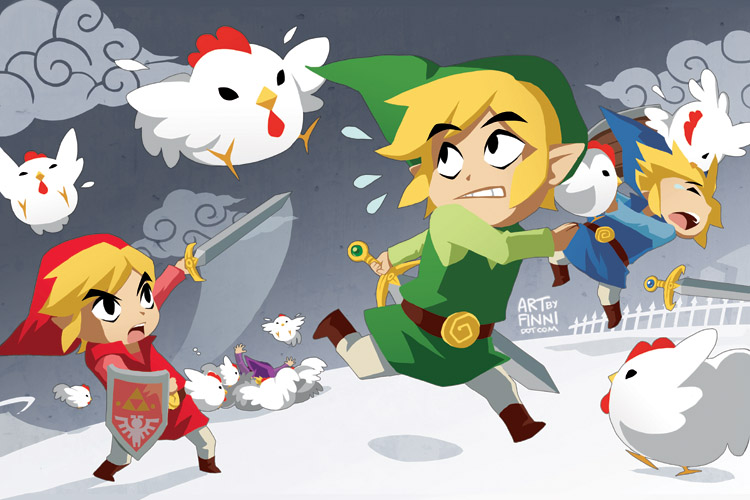
\includegraphics[width=0.6\textwidth]{figures/Sample/tumblr_static_eaceks0rfxsss8o4swscw40wo.jpg}
    \caption[Single Figure Environment Listed Title]{This is a single figure 
    environment}
    \label{fig_singleenv}
\end{figure}

This is a multi-image figure with a top (Figure~\ref{fig_multienv_1}) and bottom (Figure~\ref{fig_multienv_2}) aligned subfigures:

\begin{figure}[ht]
	\centering
	\begin{subfigure}[t]{\textwidth}
		\centering
		
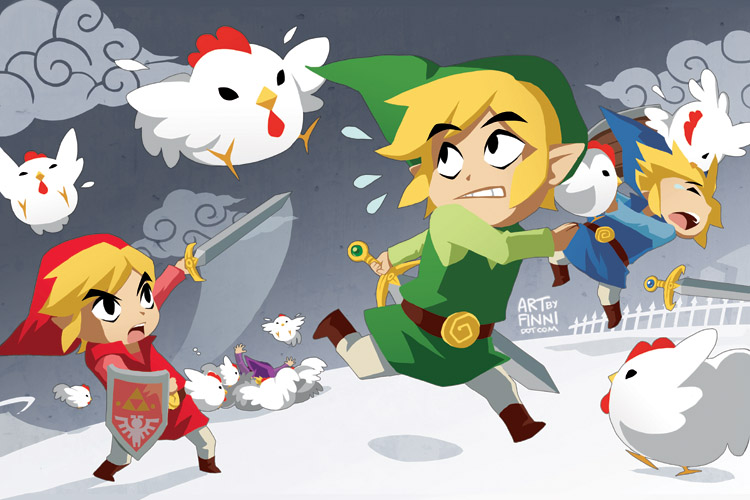
\includegraphics[width=0.7\textwidth]{figures/Sample/tumblr_static_eaceks0rfxsss8o4swscw40wo.jpg}
		\caption{Figure 1}
		\label{fig_multienv_1}
	\end{subfigure}
	~
	\begin{subfigure}[t]{\textwidth}
		\centering
		
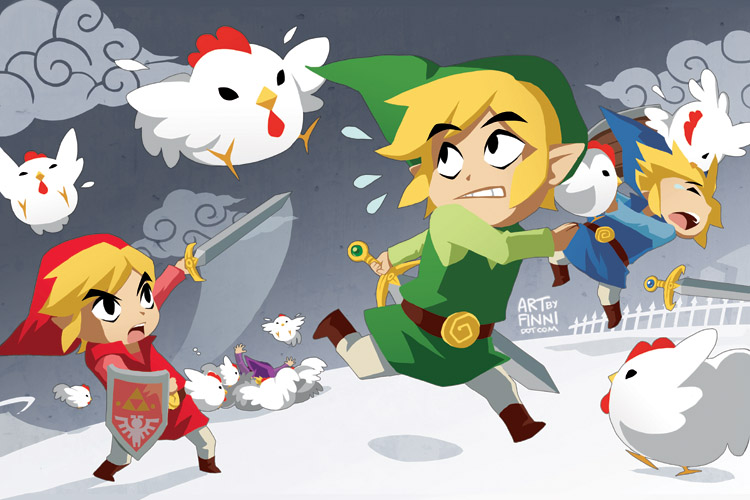
\includegraphics[width=0.7\textwidth]{figures/Sample/tumblr_static_eaceks0rfxsss8o4swscw40wo.jpg}
		\caption{Figure 2}
		\label{fig_multienv_2}
	\end{subfigure}
	
	\caption{A Multi-Figure Environment}
	\label{fig_multienv}
\end{figure}

\section{Tables}

Here is a sample table (Table~\ref{tab_sample}):

	\begin{table}[ht]
	\centering
	\begin{tabular}{ m{0.2\textwidth} m {0.1\textwidth} m{0.15\textwidth} }
		\toprule
		A & $\longleftrightarrow$ & B \\
		C & $\longleftrightarrow$ & D \\
		\bottomrule	
	\end{tabular}	
	\caption{A sample table}	
	\label{tab_sample}
\end{table}

\subsection{Long Tables}
A sample long table is shown in Appendix~\ref{appendix_b}.

\section{Equations}

Here is a sample equation (Equation~\ref{eq_lineslope}):

\begin{equation} \label{eq_lineslope}
	y = mx + b
=======
<<<<<<< HEAD
\chapter{Your Chapter Title}

This is a sample chapter

If you need to use quotes, type it ``like this''.

\section{Referencing}
These are some sample references to GAMYGDALA~\citep{popescu2014gamygdala} from 
the \texttt{references.bib} file and state effects of 
cognition~\citep{hudlicka2002time} from the \texttt{references\_another.bib} 
file. These references are not in the same .bib file.

\section{Figures}
This is a single image figure (Figure~\ref{fig_singleenv}):

\begin{figure}[ht]
    \centering
    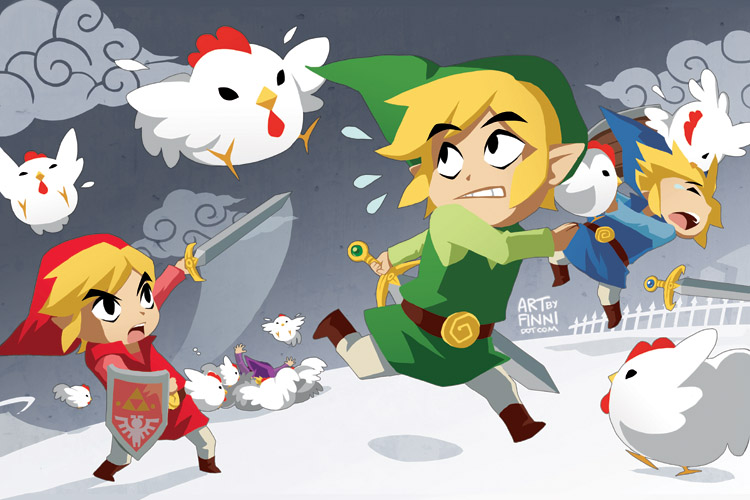
\includegraphics[width=0.6\textwidth]{figures/Sample/tumblr_static_eaceks0rfxsss8o4swscw40wo.jpg}
    \caption[Single Figure Environment Listed Title]{This is a single figure 
    environment}
    \label{fig_singleenv}
\end{figure}

This is a multi-image figure with a top (Figure~\ref{fig_multienv_1}) and bottom (Figure~\ref{fig_multienv_2}) aligned subfigures:

\begin{figure}[ht]
	\centering
	\begin{subfigure}[t]{\textwidth}
		\centering
		
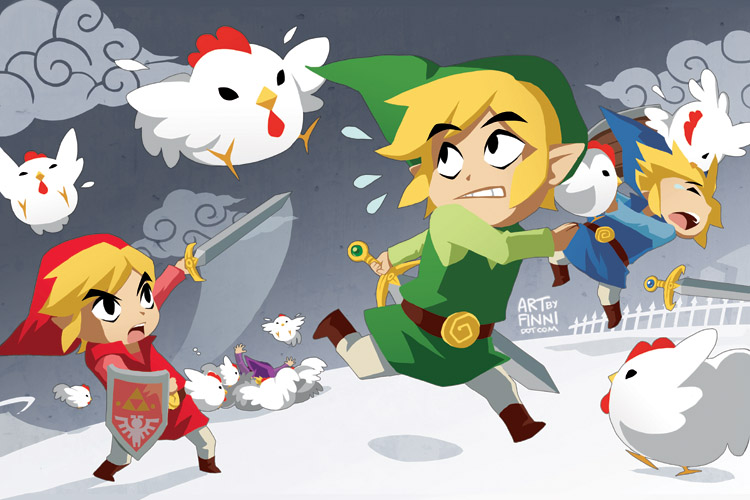
\includegraphics[width=0.7\textwidth]{figures/Sample/tumblr_static_eaceks0rfxsss8o4swscw40wo.jpg}
		\caption{Figure 1}
		\label{fig_multienv_1}
	\end{subfigure}
	~
	\begin{subfigure}[t]{\textwidth}
		\centering
		
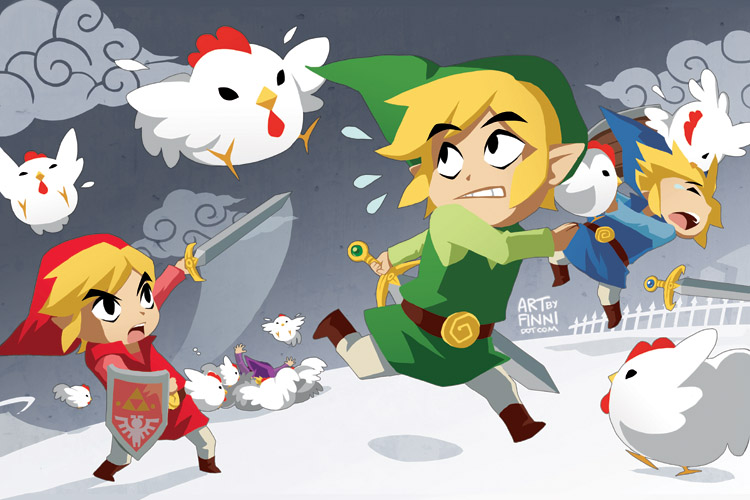
\includegraphics[width=0.7\textwidth]{figures/Sample/tumblr_static_eaceks0rfxsss8o4swscw40wo.jpg}
		\caption{Figure 2}
		\label{fig_multienv_2}
	\end{subfigure}
	
	\caption{A Multi-Figure Environment}
	\label{fig_multienv}
\end{figure}

\section{Tables}

Here is a sample table (Table~\ref{tab_sample}):

	\begin{table}[ht]
	\centering
	\begin{tabular}{ m{0.2\textwidth} m {0.1\textwidth} m{0.15\textwidth} }
		\toprule
		A & $\longleftrightarrow$ & B \\
		C & $\longleftrightarrow$ & D \\
		\bottomrule	
	\end{tabular}	
	\caption{A sample table}	
	\label{tab_sample}
\end{table}

\subsection{Long Tables}
A sample long table is shown in Appendix~\ref{appendix_b}.

\section{Equations}

Here is a sample equation (Equation~\ref{eq_lineslope}):

\begin{equation} \label{eq_lineslope}
	y = mx + b
=======
\chapter{Your Chapter Title}

This is a sample chapter

If you need to use quotes, type it ``like this''.

\section{Referencing}
These are some sample references to GAMYGDALA~\citep{popescu2014gamygdala} from 
the \texttt{references.bib} file and state effects of 
cognition~\citep{hudlicka2002time} from the \texttt{references\_another.bib} 
file. These references are not in the same .bib file.

\section{Figures}
This is a single image figure (Figure~\ref{fig_singleenv}):

\begin{figure}[ht]
    \centering
    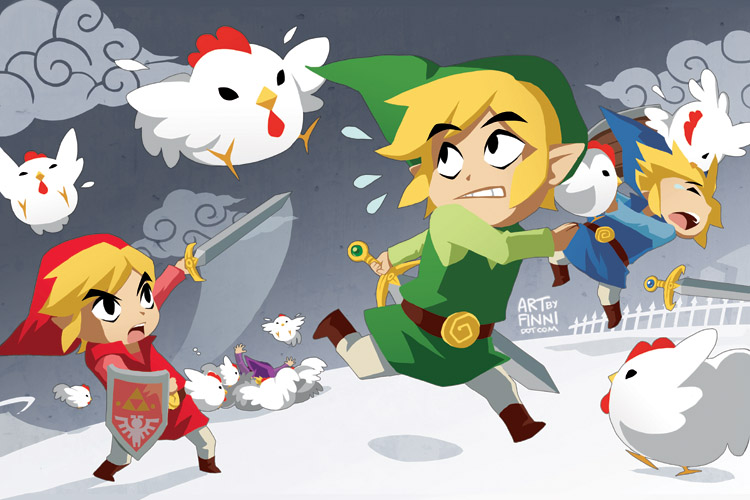
\includegraphics[width=0.6\textwidth]{figures/Sample/tumblr_static_eaceks0rfxsss8o4swscw40wo.jpg}
    \caption[Single Figure Environment Listed Title]{This is a single figure 
    environment}
    \label{fig_singleenv}
\end{figure}

This is a multi-image figure with a top (Figure~\ref{fig_multienv_1}) and bottom (Figure~\ref{fig_multienv_2}) aligned subfigures:

\begin{figure}[ht]
	\centering
	\begin{subfigure}[t]{\textwidth}
		\centering
		
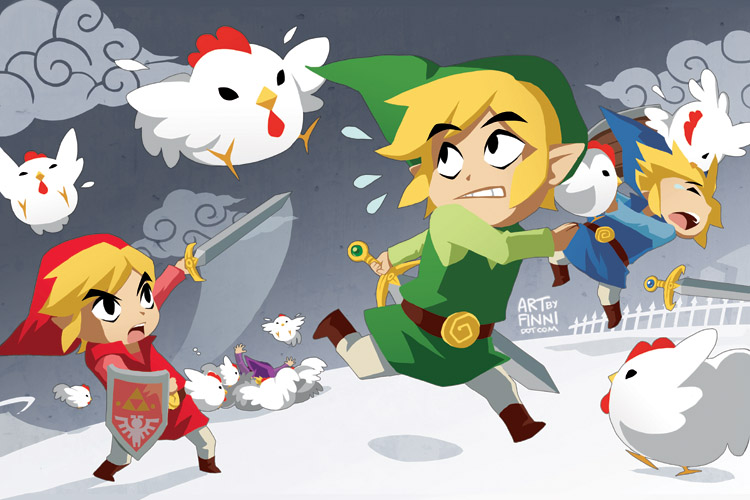
\includegraphics[width=0.7\textwidth]{figures/Sample/tumblr_static_eaceks0rfxsss8o4swscw40wo.jpg}
		\caption{Figure 1}
		\label{fig_multienv_1}
	\end{subfigure}
	~
	\begin{subfigure}[t]{\textwidth}
		\centering
		
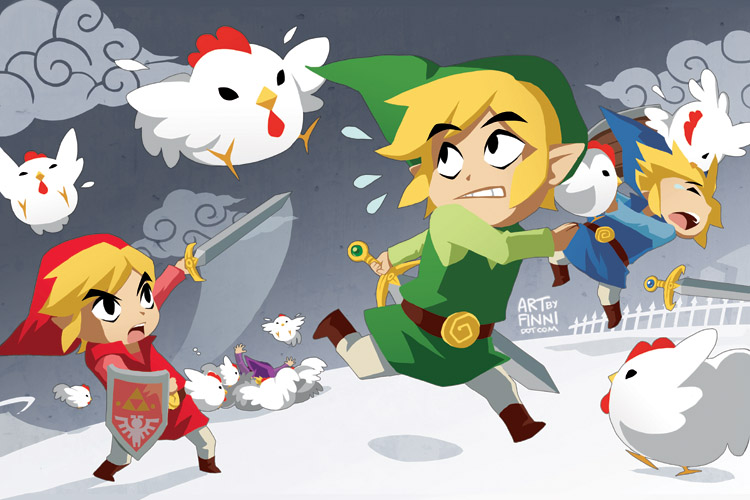
\includegraphics[width=0.7\textwidth]{figures/Sample/tumblr_static_eaceks0rfxsss8o4swscw40wo.jpg}
		\caption{Figure 2}
		\label{fig_multienv_2}
	\end{subfigure}
	
	\caption{A Multi-Figure Environment}
	\label{fig_multienv}
\end{figure}

\section{Tables}

Here is a sample table (Table~\ref{tab_sample}):

	\begin{table}[ht]
	\centering
	\begin{tabular}{ m{0.2\textwidth} m {0.1\textwidth} m{0.15\textwidth} }
		\toprule
		A & $\longleftrightarrow$ & B \\
		C & $\longleftrightarrow$ & D \\
		\bottomrule	
	\end{tabular}	
	\caption{A sample table}	
	\label{tab_sample}
\end{table}

\subsection{Long Tables}
A sample long table is shown in Appendix~\ref{appendix_b}.

\section{Equations}

Here is a sample equation (Equation~\ref{eq_lineslope}):

\begin{equation} \label{eq_lineslope}
	y = mx + b
>>>>>>> 9d845fd9678a4217417e588c8e1f2a2f78b24c2f
>>>>>>> Stashed changes
\end{equation}                  
       \setcounter{figure}{0}
       \setcounter{equation}{0}
       \setcounter{table}{0}

  <<<<<<< Updated upstream
\chapter{Conclusion}

=======
<<<<<<< HEAD
\chapter{Conclusion}

=======
\chapter{Conclusion}

>>>>>>> 9d845fd9678a4217417e588c8e1f2a2f78b24c2f
>>>>>>> Stashed changes
Every thesis also needs a concluding chapter
        \setcounter{figure}{0}
        \setcounter{equation}{0}
        \setcounter{table}{0}

\begin{appendix}
    <<<<<<< Updated upstream
\chapter{Your Appendix}
\label{appendix_a}

Your appendix goes here.
=======
<<<<<<< HEAD
\chapter{Your Appendix}
\label{appendix_a}

Your appendix goes here.
=======
\chapter{Your Appendix}
\label{appendix_a}

Your appendix goes here.
>>>>>>> 9d845fd9678a4217417e588c8e1f2a2f78b24c2f
>>>>>>> Stashed changes

        \setcounter{figure}{0}
        \setcounter{equation}{0}
        \setcounter{table}{0}

    <<<<<<< Updated upstream
\chapter{Long Tables}
\label{appendix_b}

This appendix demonstrates the use of a long table that spans multiple pages.

\begin{center}
\begin{longtable}{P{3cm}P{3cm}P{2.5cm}P{3.5cm}}
\toprule
\hline
\textbf{Col A} & \textbf{Col B} & \textbf{Col C} & \textbf{Col D} \\ \midrule

\endfirsthead
\multicolumn{4}{c}{\textit{Continued from previous page}} \\ \hline
\textbf{Col A} & \textbf{Col B} & \textbf{Col C} & \textbf{Col D} \\ \hline
\endhead
\hline \multicolumn{4}{r}{\textit{Continued on the next page}} \\
\endfoot
\hline
\endlastfoot

A & B & C & D \\ \midrule

A & B & C & D \\ \midrule

A & B & C & D \\ \midrule

A & B & C & D \\ \midrule

A & B & C & D \\ \midrule

A & B & C & D \\ \midrule

A & B & C & D \\ \midrule

A & B & C & D \\ \midrule

A & B & C & D \\ \midrule

A & B & C & D \\ \midrule

A & B & C & D \\ \midrule

A & B & C & D \\ \midrule

A & B & C & D \\ \midrule

A & B & C & D \\ \midrule

A & B & C & D \\ \midrule

A & B & C & D \\ \midrule

A & B & C & D \\ \midrule

A & B & C & D \\ \midrule

A & B & C & D \\ \midrule

A & B & C & D \\ \midrule

\hline
\end{longtable}
\end{center}
=======
<<<<<<< HEAD
\chapter{Long Tables}
\label{appendix_b}

This appendix demonstrates the use of a long table that spans multiple pages.

\begin{center}
\begin{longtable}{P{3cm}P{3cm}P{2.5cm}P{3.5cm}}
\toprule
\hline
\textbf{Col A} & \textbf{Col B} & \textbf{Col C} & \textbf{Col D} \\ \midrule

\endfirsthead
\multicolumn{4}{c}{\textit{Continued from previous page}} \\ \hline
\textbf{Col A} & \textbf{Col B} & \textbf{Col C} & \textbf{Col D} \\ \hline
\endhead
\hline \multicolumn{4}{r}{\textit{Continued on the next page}} \\
\endfoot
\hline
\endlastfoot

A & B & C & D \\ \midrule

A & B & C & D \\ \midrule

A & B & C & D \\ \midrule

A & B & C & D \\ \midrule

A & B & C & D \\ \midrule

A & B & C & D \\ \midrule

A & B & C & D \\ \midrule

A & B & C & D \\ \midrule

A & B & C & D \\ \midrule

A & B & C & D \\ \midrule

A & B & C & D \\ \midrule

A & B & C & D \\ \midrule

A & B & C & D \\ \midrule

A & B & C & D \\ \midrule

A & B & C & D \\ \midrule

A & B & C & D \\ \midrule

A & B & C & D \\ \midrule

A & B & C & D \\ \midrule

A & B & C & D \\ \midrule

A & B & C & D \\ \midrule

\hline
\end{longtable}
\end{center}
=======
\chapter{Long Tables}
\label{appendix_b}

This appendix demonstrates the use of a long table that spans multiple pages.

\begin{center}
\begin{longtable}{P{3cm}P{3cm}P{2.5cm}P{3.5cm}}
\toprule
\hline
\textbf{Col A} & \textbf{Col B} & \textbf{Col C} & \textbf{Col D} \\ \midrule

\endfirsthead
\multicolumn{4}{c}{\textit{Continued from previous page}} \\ \hline
\textbf{Col A} & \textbf{Col B} & \textbf{Col C} & \textbf{Col D} \\ \hline
\endhead
\hline \multicolumn{4}{r}{\textit{Continued on the next page}} \\
\endfoot
\hline
\endlastfoot

A & B & C & D \\ \midrule

A & B & C & D \\ \midrule

A & B & C & D \\ \midrule

A & B & C & D \\ \midrule

A & B & C & D \\ \midrule

A & B & C & D \\ \midrule

A & B & C & D \\ \midrule

A & B & C & D \\ \midrule

A & B & C & D \\ \midrule

A & B & C & D \\ \midrule

A & B & C & D \\ \midrule

A & B & C & D \\ \midrule

A & B & C & D \\ \midrule

A & B & C & D \\ \midrule

A & B & C & D \\ \midrule

A & B & C & D \\ \midrule

A & B & C & D \\ \midrule

A & B & C & D \\ \midrule

A & B & C & D \\ \midrule

A & B & C & D \\ \midrule

\hline
\end{longtable}
\end{center}
>>>>>>> 9d845fd9678a4217417e588c8e1f2a2f78b24c2f
>>>>>>> Stashed changes

        \setcounter{figure}{0}
        \setcounter{equation}{0}
        \setcounter{table}{0}
\end{appendix}

% The bibliography is set up to allow for multiple bib files
\bibliographystyle{ACM-Reference-Format}
\bibliography{references,references_another}

\label{NumDocumentPages}

\end{document}
% ********************************
>>>>>>> 9d845fd9678a4217417e588c8e1f2a2f78b24c2f
>>>>>>> Stashed changes
